
\section{Efficient Algorithms: Primes and Factoring}

The input of the primality problem is the binary representation of $n$, of size $N = \log_2 n$
bits. An algorithm is \textbf{efficient} if it runs in time polynomial in $N$.

Trial division takes $\bigTh{\sqrt{n}} = \bigTh{2^{N/2}}$ time, which is exponential. A deterministic
polynomial-time algorithm exists ($\tilde{\mathcal{O}}(N^{6})$) but is not used in practice. The
\emph{randomized} Miller--Rabin test takes $\bigO{N^3}$ time: a composite $n$ has at least
$\sfrac{3}{4}$ of $\set{2, \dots, n-2}$ as \emph{witnesses} and a prime has none, so $k$ independent
samples miss a composite with probability at most $\left(\sfrac{1}{4}\right)^k$.

\paragraph{Factoring.} Given $n = pq$ with $p, q$ prime, find $p$ and $q$. Factoring is an
\emph{encryption primitive}. No polynomial-time classical algorithm is known, but \emph{Shor's
factoring algorithm} is a quantum algorithm with running time $\bigO{N^3}$. No quantum algorithm is
known that solves \nptime-complete problems such as 3-SAT in polynomial time.

\section{Random Sampling}

A randomized algorithm only needs to \emph{sample}, and a (fair) coin flip is an $\bigO{1}$ time
primitive. In an array with $n$ slots (\cref{fig:coinflips-0825}), $n$ a power of $2$, every index
has $\log n$ bits. One coin flip per bit samples a uniformly random element in $\bigO{\log n}$ time,
since $\prob{\text{index $i$ is chosen}} = \left(\sfrac{1}{2}\right)^{\log n} = \sfrac{1}{n}$.

\begin{figure}[ht]
    \centering
    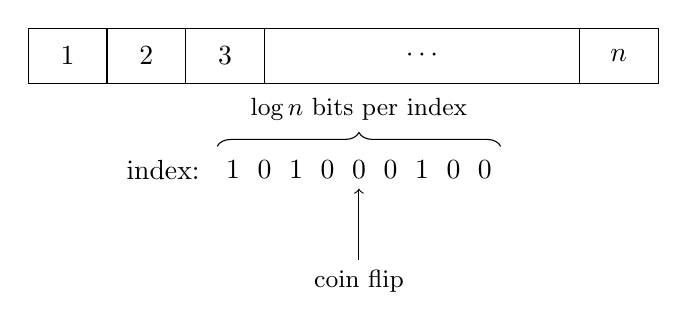
\begin{tikzpicture}
        \draw (0,0) rectangle (8,0.7);
        \foreach \x in {1,2,3,7} {\draw (\x,0) -- (\x,0.7);}
        \node at (0.5,0.35) {$1$};
        \node at (1.5,0.35) {$2$};
        \node at (2.5,0.35) {$3$};
        \node at (5,0.35) {$\cdots$};
        \node at (7.5,0.35) {$n$};
        \node[anchor=east] at (2.3,-1.1) {index:};
        \foreach \x/\b in {0/1,1/0,2/1,3/0,4/0,5/0,6/1,7/0,8/0} {
                \node (b\x) at (2.6+0.4*\x,-1.1) {$\b$};
            }
        \draw[->] (b4.south) ++(0,-0.9) -- (b4.south);
        \node[below] at (4.2,-2.25) {\small coin flip};
        \draw[decorate, decoration={brace, amplitude=5pt}] (2.4,-0.8) -- (6.0,-0.8)
        node[midway, above=6pt] {\small $\log n$ bits per index};
    \end{tikzpicture}
    \caption{Each of the $\log n$ bits of the index is one coin flip.}
    \label{fig:coinflips-0825}
\end{figure}

We sample \emph{with} replacement, so that the samples are independent. A sample hits a given
element with probability $\sfrac{1}{n}$, so finding it takes $n$ samples in expectation
(\cref{thm:geometric-0827}).

\section{Search}

An unsorted array $A$ with $n$ slots is accessed by \emph{queries} (``what is $A[i]$?''), and we
want the index of a given element $x$. Linear search makes $\bigO{n}$ queries. The lower bound uses
an \emph{adversary argument}: the adversary builds an input on which the algorithm does badly.

\begin{theorem}[Lower Bound for Deterministic Search]\label{thm:detsearch-0825}
    Every deterministic algorithm for search makes at least $n - 1$ queries in the worst case.
\end{theorem}

\begin{proof}
    Whenever the algorithm queries a slot $i$, the adversary answers that $A[i] \neq x$. The algorithm
    is deterministic, so this defines one run. Suppose that it stops after $k \leq n - 2$ queries and
    outputs an index $j$. At least $2$ slots have not been queried, so the adversary can place $x$ in
    an unqueried slot different from $j$. This array is consistent with all the answers, and the
    algorithm is wrong on it. So a correct algorithm makes at least $n - 1$ queries.
\end{proof}

Randomized search needs $\bigOm{n}$ expected queries (\emph{Yao's min-max principle}), and Grover's
quantum algorithm needs $\bigO{\sqrt{n}}$ queries. A \emph{quantum advantage} is a problem with
$\bigOm{f(n)}$ queries classically and $\littleO{f(n)}$ queries quantumly.

\section{Probability}

\begin{itemize}
    \item \textbf{Sample space:} a finite set $S$ of \emph{simple events}, $\abs{S} = n$.
    \item \textbf{Probability function:} $\Pr \colon S \to [0,1]$.
    \item \textbf{Event:} a subset $A \subseteq S$, with $\prob{A} = \sum_{a \in A} \prob{a}$.
    \item \textbf{Axioms:} $\prob{A} \geq 0$, $\prob{S} = 1$, and
          $\prob{A_1 \cup \dots \cup A_n} = \sum_{i=1}^{n} \prob{A_i}$ for pairwise disjoint events.
    \item \textbf{Random variable:} a function $X \colon S \to V$, with
          $\prob{X = r} = \sum_{s \in S \,:\, X(s) = r} \prob{s}$.
\end{itemize}
